\documentclass[12pt]{article}

\usepackage[T1]{fontenc}
\usepackage[utf8]{inputenc}
\usepackage[russian]{babel}
\usepackage{xcolor}
\usepackage{minted}
\usepackage{graphicx}
\usepackage{float}
\usepackage[margin=1.5cm]{geometry}

\setlength{\parindent}{1.25cm}

\newminted{python}
{
    frame=lines,
    framesep=2mm,
    baselinestretch=1.2,
    bgcolor=darkgray,
    fontsize=\footnotesize,
    python3,
    style=monokai,
    rulecolor=white
}

\title{Разбор задач конкурса "Звезды Кассиопеи"}
\date{20.05.2021}
\author{Надобных Дмитрий, Пугач Сергей, Чечеватов Роман}

\begin{document}
    \pagenumbering{gobble}
    \maketitle
    \pagenumbering{arabic}
    \newpage
    \raggedright


    \section{Ручные задачи}

    \paragraph{}
    Для решения данных задач не нужны никакие навыки программирования и они вам не сильно помогут.
    Вместо этого участникам предлагалось научиться искать информацию в файлах, анализировать их.
    \newpage

    \subsection{MP5}

    \paragraph{}
    Эта задача засчитывалась как решенная после перехода по ссылке.
    Ничего сложного.

    % \newpage

    \subsection{Автостоп}
    \paragraph{}
    Как сказано в условии, ответом на данную задачу является ответ на Главный вопрос жизни, вселенной и всего такого.
    Вопрос этот был задан английским писателем Дугласом Адамсом в книге \verb|"The Hitchhiker’s Guide to the Galaxy"|,
    русским читателям известной как \verb|"Автостопом по галактике"|.
    \paragraph{}
    Участники, читавшие этот роман могут спокойно ответить \verb|42| и получить баллы,
    остальным придется скопировать вопрос в Гугл и получить ответ в первом же результате.
    \paragraph{}
    Ответ: \verb|42|

    % \newpage

    \subsection{Язык программирования}
	\paragraph{}
    Для решения этой задачи участникам необходимо было изучить HTML-код страницы задачи.
	Для этого можно воспользоваться встроенными в браузер инструментами разработчика,
	или скачать страницу и открыть в текстовом редакторе.
	\paragraph{}
	Независимо от выбранного способа, ответ находился в комментарии рядом с формой ввода ответа.
    \paragraph{}
    Ответ: \verb|flag{html_is_the_best_language}|

    % \newpage

    \subsection{Фотосессия}
	\paragraph{}
    В данной задаче участникам давался для анализа JPG-файл с картинкой.
	Однако, такие файлы зачастую содержат в себе не только данные изображения, но и дополнительную информацию.
	Например, дату съемки, модель камеры, имя автора.
	И среди этой дополнительной информации и был спрятан флаг.
    \paragraph{}
    Ответ: \verb|flag{haha_you_thought_it_will_be_ccv}|

    % \newpage

    \subsection{PI}
	\paragraph{}
    Здесь участников просили ввести число Пи с некоторой точностью:
	строго заданное число знаков после запятой, не больше и не меньше.
	Достаточно точное число Пи можно взять на Википедии или, для пользователей Windows 10, Калькуляторе.
    \paragraph{}
    Отгадать необходимую точность можно с помощью метода проб и ошибок, или просто написав бота.
    \paragraph{}
    Ответ: \verb|3.14159265358979323846264338327|

    % \newpage

    \subsection{Задача, которую невозможно решить}
	\paragraph{}
    Вопреки сказанному в названии задачи, ее возможно решить.
	Наличие решения этой задачи показывает,
	как внимательно участники прочитали инструкцию по работе с тестирующей системой.
	Ведь именно в разделе \verb|Мануал|, в подразделе \verb|Обработка персональных данных|,
	совершенно не к месту находилось предложение
    \verb|Однако, для решения задачи, которую невозможно решить, вам нужно всего лишь отправить название конкурса|.
	Остается лишь найти правильное с точностью до символа название.
    \paragraph{}
    Ответ: \verb|Звезды Кассиопеи|

    % \newpage

    \subsection{Двадцать пятый кадр}
	\paragraph{}
    В данной задаче участникам предлагался для анализа файл с видео.
	И хотя в метаданных на этот раз флага не было, там можно было обнаружить частоту кадров видео: 120~кадров в секунду.
	Это значит, что на экранах с частотой обновления 60~Гц и менее
	(а таких на момент проведения конкурсов подавляющее большинство)
	немалая часть кадров просто не будет отображаться.
	Но зачем же авторы дали видео с таким большим числом кадров, зная, что часть из них не будет показана?
	Неужели они хотели что-то там спрятать?
	Да.
	Смотрим видео покадрово и на 817~кадре замечаем серый текст на сером фоне.
    \paragraph{}
    Ответ: \verb|flag{you_have_great_eyes}|

    % \newpage

    \subsection{Eglishman}
	\paragraph{}
    В очередной раз отправляемся в Гугл (Яндекс, Bing, DuckDuckGo, Рамблер, Поиск~Маил.Ру,~\ldots)
	чтобы узнать, как сервер может узнать местоположение/страну/язык пользователя и узнаем, два основных способа:
	по~IP и по предпочитаемому языку пользователя.
    \paragraph{}
	Методом проб и ошибок, испробовав все платные и бесплатные VPN-сервера узнаем,
	что в данной задаче IP ничего не значит.
    \paragraph{}
	Остается вариант с языком.
	Браузер внутри запроса отправляет информацию о предпочитаемом языке веб-страниц.
	В настройках браузера выставляем предпочтение на английский, отправляем что угодно в качестве ответа и получаем баллы.

    % \newpage

    \subsection{1C}
	\paragraph{}
    В следующей задаче на анализ содержимого файла участникам был дан файл Excel.
	Изучив свойства файла или создав новый лист, можно обнаружить,
	что кроме видимого листа с многозначащим названием \verb|Лист1| в книге есть еще два: \verb|Лист2| и \verb|Лист3|.
	В Microsoft Office Excel жмем ПКМ по списку листов, \verb|Показать...|, \verb|Лист3|.
	Изучаем содержимое ранее скрытого листа рядом с красивой картинкой аэродинамических характеристик коровы
	обнаруживаем флаг.
    \paragraph{}
    Ответ: \verb|flag{cow_aerodynamics_power}|

    % \newpage

    \subsection{Машина времени}
	\paragraph{}
    Снова скачиваем приложенный файл.
	Распаковываем архив, наряду с привычными, но ничем не примечательными файлами обнаруживаем папку \verb|.git|.
	Или не обнаруживаем, если у вас не включено отображение скрытых файлов.
	В таком случае, включаем, потому что без него заниматься поиском скрытой информации весьма непросто.
    \paragraph{}
	В любом случае, закинув название папки в Гугл получаем понимание, что авторы дали вам Git-репозиторий.
	Git - одна из систем контроля версий, то есть позволяет отслеживать и сохранять изменения файлов,
	откатываться к предыдущей версии.
    \paragraph{}
	Скачиваем Git, устанавливаем.
	Делаем коммит с помощью \verb|git commit -a|, видим, что после последнего коммита (сохранения) файлы изменялись.
	Откатываемся к предыдущему коммиту \verb|git checkout a23d2c7|,
    смотрим содержимое когда-то бывшего удаленным файла, находим флаг.
    \paragraph{}
    Ответ: \verb|flag{wayback_machine_master}|

    % \newpage

    \subsection{Пленочный фотоаппарат}
    \paragraph{}
    % TODO
    \paragraph{}
    Ответ: \verb|flag{that_was_a_good_2.3BTC}|
    % \newpage

    \subsection{Пленочный фотоаппарат 2}
    \paragraph{}
    % TODO
    \paragraph{}
    Ответ: \verb|flag{that_was_my_last_money}|

    \newpage

    \section{Задачи на использование ботов}
	\paragraph{}
    Для начала рассмторим общую для всех ботов часть: работу с сетью.
	Мы использовали для написания ботов \verb|Python 3| и библиотеку \verb|requests|.
	Ничто не мешало вам использовать другие варианты,
	а незнание любого из них компенсируется длиной конкурса и доступностью все того же Гугла.
	\paragraph{}
    Импортируем библиотеку и задаем константы:
    \begin{pythoncode}
# -*- coding: utf-8 -*- # Волшебное слово, чтобы использовать кириллицу
import requests # Импортируем requests

login = 'login' # Сохраняем логин и токен
token = '23847634320439b65adafb7e3fefff802b1cde0a1b2977c3fe299a6dd111e4ce'
host = 'https://fetefot763.eu.pythonanywhere.com/'
    \end{pythoncode}

    Теперь нужно разобраться, как браузер отправляет запросы на сайт.
    Открываем панель разработчика и изучаем (смотри рисунок~\ref{fig:browser1}):
    \begin{figure}[H]
        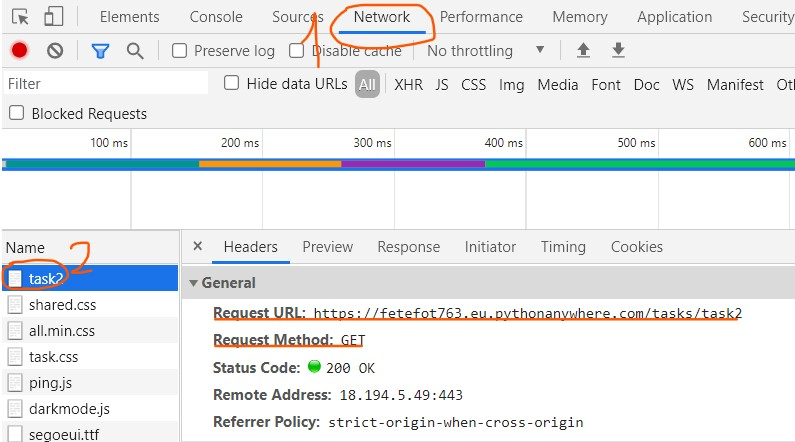
\includegraphics[width=\linewidth]{BrowserNetworkAnalysis0}
        \caption{Изучение процесса получения страницы браузером.}
        \label{fig:browser1}
    \end{figure}

    Видим, что браузер отправляет GET-запрос на страницу задачи.
    Продолжаем изучение, проматываем вниз (смотри~рисунок~\ref{fig:browser2}):

    \begin{figure}[H]
        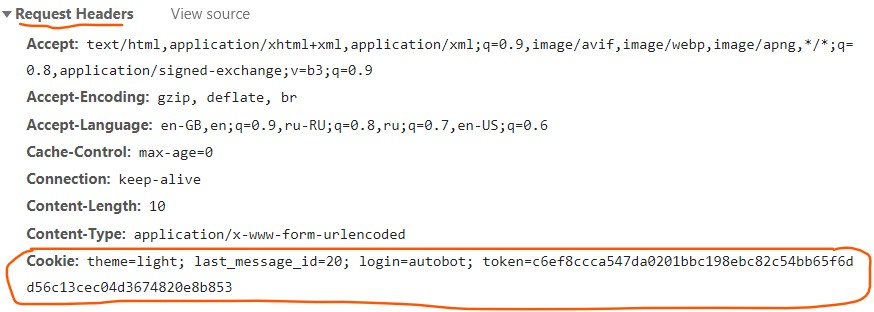
\includegraphics[width=\linewidth]{BrowserNetworkAnalysis2}
        \caption{Изучение отправляемых браузером cookie-файлов.}
        \label{fig:browser2}
    \end{figure}

    Теперь видим, что браузер отправляет cookie-файлы, чтобы получить страницу.
    Почитав в мануале обнаруживаем, что для работы необходимо только две печеньки: \verb|login| и \verb|token|.
    Их значения сохраняем к себе и используем дальше.
    \paragraph{}
    Используя полученные знания мы можем написать функцию получения задачи.
    Функция - это обособленный фрагмент кода, выполняющий узкую задачу.
    \paragraph{}
    Для задач, где в приложении дан текст, мы можем получить этот текст прямо со страницы задачи:

    \begin{pythoncode}
# Для текстовых задач (на примере задачи №1 - Водолей)
def get_data(): # Объявляем функцию
    text = requests.get(                          # Отправляем запрос
        host + 'tasks/task1',                     # На страницу задачи
        cookies={'login': login, "token": token}  # С cookies авторизации
    ).text # И сохраняем текст ответа в переменную text
    return text # Возвращаем text
    \end{pythoncode}

    \paragraph{}
    Заметим, что функция \verb|get_data| возвращает нам весь HTML-код страницы.
    Нам же нужно только приложение к заданию.
    Приложения всегда находятся в блоке с \verb|id="task_data"| и не содержат блоков внутри.
    Пользуясь этим, создадим новую функцию для извлечения этого приложения:

    \begin{pythoncode}
def get_text_from_data(data):
    marker_beg = '<div id="task-data">'
    marker_end = '</div>'
    ind_beg = data.rfind(marker_beg) + len(marker_beg)  # Индекс начала содержимого блока в строке
    ind_end = data[ind_beg:].find(marker_end)           # Индекс конца содержимого блока в строке
    text = data[ind_beg:ind_beg + ind_end]              # Сохраняем содержимое блока в переменную
    return text # Возвращаем text
    \end{pythoncode}

    Следует четко понимать, какую задачу вы решаете и какие функции из приложенных вам следует использовать.
    Так, функция получения текста задачи вернет мусор, если текста в задаче не окажется.
    А что произойдет с вашей программой при попадании внутрь мусора никому не известно.
    \paragraph{}
    Если же в приложении дана ссылка на файл, то его нужно скачать.
    Тогда функция может ничего не возвращать: результат запроса уже сохранен в файл и будет прочитан из него.

    \begin{pythoncode}
# Для файловых задач (на примере задачи №2 - WinRar 3000)
def get_data(): # Объявляем функцию
    requests.get(                                 # Отправляем запрос
        host + 'tasks/task2',                     # На страницу задачи
        cookies={'login': login, "token": token}  # С cookies авторизации
    )
    with open('2.zip', 'wb') as file: # Создаем и открываем файл 2.zip для записи
        file.write(                               # Записываем в файл
            requests.get(                         # Отправляем запрос
                host + f'task-generated-content/2/task2_{team_id}.zip', # За файлом
                cookies={'login': login, "token": token} # С cookies авторизации
            ).content # Записываем в файл ответ на запрос
        )
    \end{pythoncode}

    \paragraph{}
    Теперь проанализируем отправку браузером нашего решения задачи.
    Напишем что-нибудь в поле ответа и нажмем кнопку отправки.
    Посмотрим, что же нам показывает браузер в уже знакомой панели (смотри~рисунок~\ref{fig:browser3}):

    \begin{figure}[H]
        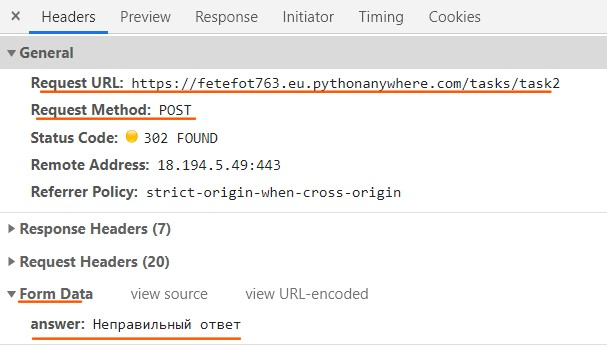
\includegraphics[width=\linewidth]{BrowserNetworkAnalysis3}
        \caption{Изучение отправки браузером ответа на задачу.}
        \label{fig:browser3}
    \end{figure}

    \paragraph{}
    Видим, что браузер отправляет запрос все на ту же страницу, но уже POST-запрос.
    В запрос браузер включает \verb|данные формы|, содержащие поле \verb|answer| со значением,
    которое мы только что вписали в поле ввода ответа.
    Как всегда, cookie браузер тоже отправляет.
    \paragraph{}
    Напишем функцию отправки ответа в данных формы:

    \begin{pythoncode}
def send_data(data): # Объявляем функцию
    requests.post(                                # Отправляем запрос
        host + f'tasks/task{task_id}',            # На страницу задачи
        data={'answer': data},                    # С данными формы
        cookies={'login': login, "token": token}  # И cookies авторизации
    )
    \end{pythoncode}

    \paragraph{}
    На этом работа с сетью завершается.
    Остается только в правильном порядке вызывать наши функции:

    \begin{pythoncode}
# Для текстовых задач
if __name__ == '__main__': # Если запущен именно этот файл
    while True: # Вечный цикл
        txt = get_text_from_data(get_data())      # Получаем текст задачи
        res = solve(txt)                          # Решаем задачу и сохраняем ответ
        send_data(res)                            # Отправляем ответ
    \end{pythoncode}

    \begin{pythoncode}
# Для файловых задач
if __name__ == '__main__': # Если запущен именно этот файл
    while True: # Вечный цикл
        get_data()                                # Получаем данные
        res = solve()                             # Решаем задачу и сохраняем ответ
        send_data(solve())                        # Отправляем ответ
    \end{pythoncode}

    \paragraph{}
    Просто вставить этот код себе и запустить у вас не получится: функция \verb|solve| не определена.
    Реализацию этой функции мы рассмортим отдельно для каждой задачи.

    \newpage


    \subsection{Школьный конкурс компьютерной графики на тему "Программирование"}
    \paragraph{}
    Здесь ничего решать не нужно, нужно просто отправить \verb|29 апреля|.
    Тогда фукция \verb|solve| может просто возвращать эту строку, без каких-либо вычислений.
    \begin{pythoncode}
def solve(txt):
    return '29 апреля'
    \end{pythoncode}

    % \newpage

    \subsection{Водолей}

    % \newpage

    \subsection{WinRar 3000}
    \paragraph{}
    Решаем задачу как файловую, скачиваем архив \verb|2.zip|.
    Гуглим, как с помощью утилит командной строки на Windows распаковать архив, находим команду \verb|tar -x -f 2.zip|.
    Гуглим, как с помощью Python запустить утилиту командной строки, находим библиотеку \verb|subprocess|.
    Гуглим инструкции, соединяем, пишем код:
    \begin{pythoncode}
def solve() -> str:
    subprocess.call(['tar',  '-x', '-f',  '2.zip'])
    with open('answer.txt', 'r') as res:
        return res.read()
    \end{pythoncode}
    % \newpage

    \subsection{Никита Егоров}
    Решаем задачу как текстовую.
    Вместо того, чтобы писать обработчик математики самому, воспользуемся плюсами Python и просто выполним
    строку с выражением.
    Полученный результат приведем к целому числу и отправим:
    \begin{pythoncode}
def solve(text: str) -> int:
    return int(eval(text))
    \end{pythoncode}

    % \newpage

    \subsection{Цветовод}

    \begin{pythoncode}
def solve() -> str:
    img = Image.open('29.png')
    pix = img.load()
    return '#' + \
           ''.join(
               map(
                   lambda colour: hex(255 - colour)[2:].upper().zfill(2),
                   pix[0, 0]
               )
           )
    \end{pythoncode}

    % \newpage

    \subsection{Кадровое агенство}

    % \newpage

    \subsection{Вечеринка}

    \begin{pythoncode}
def send_data():
    text = requests.post(
        host + 'tasks/task21',
        cookies={'login': login, 'token': token, 'tea': 'tea'})
    return text
    \end{pythoncode}

    % \newpage

    \subsection{Календарь}

    \begin{pythoncode}
def solve(text: str) -> str:
    days = datetime.datetime.strptime(text, '%d.%m.%Y').date().toordinal()
    days += 701
    return datetime.date.fromordinal(days).strftime('%d.%m.%Y')
    \end{pythoncode}
    % \newpage

    \subsection{Я - Гуль}

    % \newpage

    \subsection{Рукой подать}

    \begin{pythoncode}
class Vector():
    x: int
    y: int

    def __init__(self, x, y):
        self.x = x
        self.y = y

    def normalize(self):
        if self.x != 0: self.x = self.x // abs(self.x)
        if self.y != 0: self.y = self.y // abs(self.y)

def solve() -> str:
    img = Image.open('43.png')
    pix = img.load()
    x1, y1, x2, y2 = None, None, None, None

    for x in range(img.size[0]):
        for y in range(img.size[1]):
            if pix[x, y] == (0, 0, 0):
                if x1 is None:
                    x1 = x
                    y1 = y
                else:
                    x2 = x
                    y2 = y
    vec = Vector(x2 - x1, y2 - y1)
    vec.normalize()

    if vec.x == 1 and vec.y == 1: x1 += 1; y1 += 1
    if vec.x == -1 and vec.y == 1: y1 += 1; x2 += 1
    if vec.x == 1 and vec.y == -1: x1 += 1; y2 += 1
    if vec.x == -1 and vec.y == -1: x2 += 1; y2 += 1

    if vec.x == 0 and vec.y == 1: y1 += 1
    if vec.x == 0 and vec.y == -1: y2 += 1
    if vec.y == 0 and vec.x == 1: x1 += 1
    if vec.y == 0 and vec.x == -1: x2 += 1

    length = ((x2 - x1) ** 2 + (y2 - y1) ** 2) ** 0.5

    round_len = round(length, 5)
    if int(length) != length:
        ans = str(round_len)
    else:
        ans = str(int(round_len))
    return ans
    \end{pythoncode}
    % \newpage

%    \subsection{Emoji Warrior}
%
%    \begin{pythoncode}
%def solve(text: str) -> str:
%    return text \
%        .replace('🤣🤣🤣', 'rofl') \
%        .replace('🤣🤣', 'rofl') \
%        .replace('🤣', 'rofl') \
%        .replace('🤔🤔🤔', 'ooo_OOO') \
%        .replace('🤔🤔', 'oo_OO') \
%        .replace('🤔', 'o_O') \
%        .replace('🤑🤑🤑', '$$$_$$$') \
%        .replace('🤑🤑', '$$_$$') \
%        .replace('🤑', '$_$') \
%        .replace('🙂🙂🙂', '=)))') \
%        .replace('🙂🙂', '=))') \
%        .replace('🙂', '=)') \
%        .replace('🙁🙁🙁', '=(((') \
%        .replace('🙁🙁', '=((') \
%        .replace('🙁', '=(') \
%        .replace('😕😕😕', '=///') \
%        .replace('😕😕', '=//') \
%        .replace('😕', '=/') \
%        .replace('😑😑😑', '---_---') \
%        .replace('😑😑', '--_--') \
%        .replace('😑', '-_-') \
%        .replace('😉😉😉', ';)))') \
%        .replace('😉😉', ';))') \
%        .replace('😉', ';)') \
%        .replace('😂😂😂', 'XDDD') \
%        .replace('😂😂', 'XDD') \
%        .replace('😂', 'XD')
%    \end{pythoncode}
%
%    % \newpage
%
    \subsection{CuSo4}

    \begin{pythoncode}
with open('chemlist.txt', 'r') as chemlist:
    chem = [i[:-1].lower().split(',') for i in chemlist.readlines()]
chem.sort(key=lambda x: len(x[1]), reverse=True)
print(chem)

def solve(text: str) -> str:
    for elem in chem:
        text = text.replace(elem[1], elem[0])
    return text
    \end{pythoncode}


\end{document}